%-----------------------------------------------------------------------------%
\chapter{\babDua}
%-----------------------------------------------------------------------------%


%-----------------------------------------------------------------------------%
\section{\textit{Literature Map}}
\label{sec:literature-map}
%-----------------------------------------------------------------------------%
\textit{Literature Map} merupakan sebuah visualisasi yang memuat \textit{summary} penelitian terkait yang telah dilakukan sebelumnya. \textit{Literature Map} biasanya direpresentasikan dalam sebuah gambar, misalnya menggunakan struktur hierarki \textit{top-down} dalam mempresentasikan literatur \citep{creswell_research_2013}. Ide utama dari penggambaran \textit{literature map} adalah untuk membuat visualisasi dari penelitian terdahulu tentang sebuah topik. 

\begin{figure}[!]
	\centering
	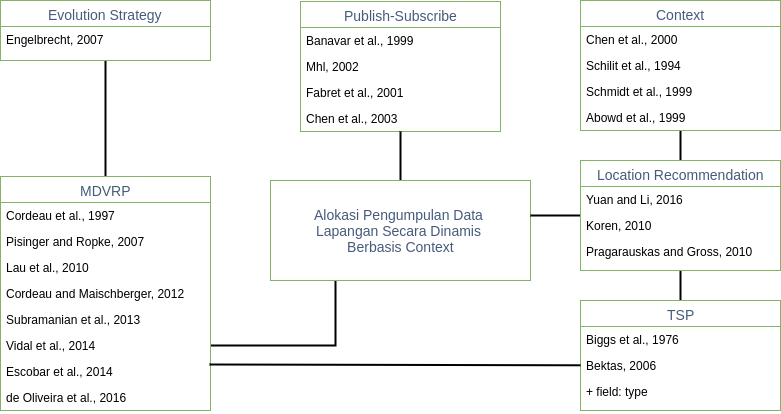
\includegraphics[width=\textwidth]{Resources/Images/literature-map}
	\captionsetup{format=hang}
	\caption{\textit{Literature Map} Penelitian}
	\label{fig:literature-map}
\end{figure}


Berdasarkan review dari literatur yang terkait dengan penelitian ini (\autoref{fig:literature-map}), arsitektur dari rekomendasi lokasi pada pengumpulan data lapangan dapat dibagi menjadi 3 (tiga) kelompok: \textit{context-aware computing}, \textit{location routing}, dan mekanisme komunikasi.


\textit{Context-aware computing} akan membahas beberapa literatur yang berkaitan dengan definisi dari konteks itu sendiri dan pemanfaatannya dalam komputasi. \textit{Location routing} akan membahas literatur terkait beberapa algoritma yang biasa digunakan dalam penyelesaian masalah \textit{location routing}. Sementara mekanisme komunikasi akan mendiskusikan tentang beberapa metode yang dapat digunakan oleh \textit{client} dan \textit{server} dalam berkormunikasi.


%-----------------------------------------------------------------------------%
\section{Badan Pusat Statistik}
\label{sec:badan-pusat-statistik}
%-----------------------------------------------------------------------------%
Badan Pusat Statistik (BPS) adalah Lembaga Pemerintah Non-Departemen yang bertanggung jawab dan memiliki peranan dalam penyediaan data. Berdasarkan Rencana Strategis BPS 2015-2019, BPS memiliki misi yang harus dijalankan yaitu:
\begin{enumerate}
\item Menyediakan data statistik berkualitas melalui kegiatan statistik yang terintegrasi dan berstandar nasional maupun internasional. \\
Dalam rangka menyediakan data berkualitas, data yang dihasilkan BPS harus memenuhi dimensi kualitas yakni relevan, akurat, disajikan tepat waktu, koheren, dapat diakses, dan dapat diinterpretasikan.
\item Memperkuat Sistem Statistik Nasional yang berkesinambungan melalui pembinaan dan koordinasi di bidang statistik.
\item Membangun insan statistik yang profesional, berintegritas dan amanah untuk kemajuan perstatistikan.
Dalam menyelenggarakan kegiatan statistik, insan statistik harus memiliki kapasitas dan kapabilitas yang diperlukan untuk menghasilkan data statistik yang berkualitas.
\end{enumerate}


Di dalam menjalankan peranan sebagai penyedia data, BPS menyelenggarakan statistik dasar dengan cara sensus, survei, dan kompilasi administrasi untuk mendapatkan data. Data yang berkualitas hanya dapat diperoleh melalui proses yang berkualitas pula. Terdapat berbagai variabel yang menjadi parameter proses yang berkualitas, salah satunya adalah ketepatan waktu dalam proses pengumpulan data.

Pengumpulan data merupakan suatu proses yang sangat fleksibel. Ketepatan waktu pengumpulan data sangat rentan terhadap pengaruh berbagai faktor, seperti kualitas petugas pengumpulan data, kualitas responden, jumlah anggota rumah tangga yang didata, jarak antar lokasi pencacahan, jarak antar rumah tangga dalam satu segmen, dan kondisi alam. Alokasi petugas pengumpulan data secara baku yang hanya memperhatikan jumlah lokasi pencacahan dan petugas, tidak dapat mengakomodir faktor-faktor tersebut. Akibatnya, waktu penyelesaian pengumpulan data bisa bervariasi antara satu petugas dengan petugas lainnya. Oleh karena itu, diperlukan suatu metode baru dalam pengalokasian petugas yang dapat mengantisipasi terjadinya kesenjangan beban tugas baik dari segi waktu maupun kuantitas.  

%-----------------------------------------------------------------------------%
\section{\textit{Context-aware Computing}}
\label{sec:context-aware-computing}
%-----------------------------------------------------------------------------%


%-----------------------------------------------------------------------------%
\subsection{Definisi \textit{Context}}
\label{ssec:context-definition}
%-----------------------------------------------------------------------------%
Semenjak \textit{Context-aware computing} pertama kali diperkenalkan oleh \citep{schilit_context-aware_1994}, berbagai definisi mengenai \textit{context} dan \textit{context-awareness} telah berkembang luas. Sebagaian besar definisi yang ada saat ini, menurut \citep{zimmermann_operational_2007}, dapat dikelompokkan menjadi dua: definisi menurut sinonim dan definisi menurut contoh. \textit{Context} mengalami berbagai penggolongan menggunakan sinonim seperti \textit{application environment} \citep{hull_towards_1997} atau situasi \citep{brown_stick-e_1995}. Sementara beberapa authors, seperti \citep{brown_context-aware_1997}, \citep{gross_awareness_2001}, dan \citep{ryan_enhanced_1999}, mendefinisikan \textit{context by example} dan \textit{context element} seperti lokasi, identitas, waktu, suhu, kebisingan sama dengan kepercayaan, keinginan, komitmen, dan hubungan dengan manusia \citep{chen_intelligent_2003}.


Secara umum, dapat dikatakan bahwasanya \textit{context} adalah informasi yang dapat digunakan dalam menjelaskan situasi dari sebuah entitas. Entitas dapat dapat berupa manusia, lokasi, atau obyek yang relevan dengan interaksi antara seorang pengguna dan aplikasi, termasuk pengguna dan aplikasi itu sendiri \citep{dey_understanding_2001}. \citep{schilit_context-aware_1994} menyebutkan bahwa yang termasuk ke dalam \textit{context} adalah: lokasi dari penggunaan, kumpulan orang-orang sekitar, \textit{hosts}, dan \textit{accessible devices}, serta perubahan hal-hal tersebut dari waktu ke waktu. \citep{dey_understanding_2001} mengembangkan definisi dari \citep{schilit_context-aware_1994} dengan menyatakan "\textit{Context} adalah lokasi, identitas dan status dari individu, kelompok, dan obyek komputasi".


%-----------------------------------------------------------------------------%
\subsection{Kategori \textit{Context}}
\label{ssec:context-category}
%-----------------------------------------------------------------------------%
Dari berbagai informasi yang menjelaskan entitas dari \textit{context}, semuanya mengarah ke 5 (lima) kategori, yaitu: \textit{individuality}, aktivitas, lokasi, waktu, dan relasi, seperti pada Gambar \ref{fig:context-categories} \citep{zimmermann_operational_2007}. Kategori \textit{individuality} memuat properti dan atribut yang menjelaskan entitas itu sendiri. Kategori aktivitas mencakup seluruh kegiatan yang dilakukan entitas tersebut. Kategori lokasi dan waktu menyediakan koordinat \textit{spatio-temporal} dari entitas. Sementara kategori relasi merepresentasikan informasi tentang hubungan antara sebuah entitas dengan entitas yang lain.


\begin{figure}[!]
	\centering
	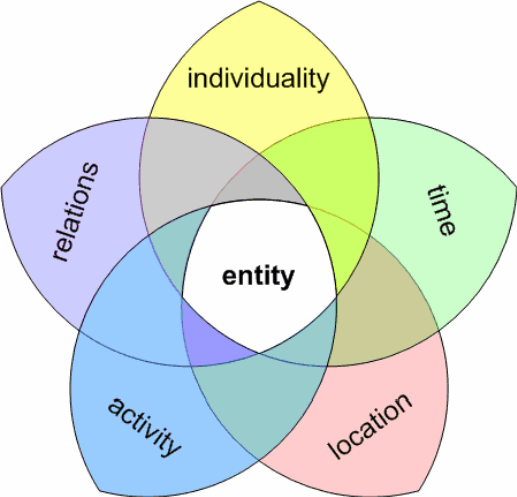
\includegraphics[width=6cm]{Resources/Images/context-categories}
	\captionsetup{format=hang}
	\caption{Kategori dari \textit{Context}}
	\label{fig:context-categories}
\end{figure}


%-----------------------------------------------------------------------------%
\subsubsection{\textit{Individuality Context}}
\label{sssec:individuality-context}
%-----------------------------------------------------------------------------%
Kategori ini memberi akses kepada informasi yang bersifat kontekstual tentang entitas terkait. Informasi ini dapat berupa apa saja terkait entitas tersebut, tetapi umumnya adalah \textit{state} dari entitas. Entitas dapat berupa entitas individu atau sekelompok entitas yang saling berbagi \textit{context} yang terkait. Entitas dapat berupa entitas yang \textit{real} (eksis secara nyata), maupun virtual (hanya terdapat di lingkup informasi). Selain itu, terdapat juga entitas yang bersifat \textit{mobile}, \textit{movable}, maupun \textit{fixed}. kategori \textit{inviduality context} dikelompokkan menjadi empat, yaitu: \textit{natural}, \textit{human}, \textit{artificial}, dan \textit{group entities}.


%-----------------------------------------------------------------------------%
\subsubsection{\textit{Time Context}}
\label{sssec:time-context}
%-----------------------------------------------------------------------------%
Waktu merupakan aspek yang vital dalam klasifikasi \textit{context}, karena sebagian besar pernyataan sangat terkait dengan dimensi \textit{temporal}. Kategori ini menkalkulasi informasi seperti \textit{time zone} dari \textit{client}, dan \textit{current time} atau \textit{virtual time}. Contoh representasi dari waktu adalah \textit{time zone}, misalnya format \textit{ Central European Time (CET)}, yang menyediakan fasilitas kalkulasi secara matematis dan komparasi waktu. Model dimensi waktu yang sering diimplementasikan dalam \textit{context-aware computing} misalnya jam kerja atau hari libur.


\textit{Context} yang disimpan secara persisten dapat membentuk sebuah \textit{data pool} yang berisi histori dari informasi terkait \textit{context} tersebut. Histori tersebut membentuk basis data untuk \textit{context information} dari event yang telah lampau. Basis data yang dipersistenkan dapa digunakan sebagai bahan analisis dari kebiasaan dari pengguna dan prediksi.


%-----------------------------------------------------------------------------%
\subsubsection{\textit{Location Context}}
\label{sssec:location-context}
%-----------------------------------------------------------------------------%
Dengan semakin berkembangnya \textit{portable/mobile devices}, lokasi menjadi parameter yang penting dalam \textit{context-aware system}. Obyek-obyek fisik dan perangkat tersusun secara spasial, dipengaruhi oleh pergerakan pengguna. Kategori ini berisi model lokasi yang terklasifikasi secara fisik maupun virtual, misalnya \textit{IP address} sebagai posisi komputer dalam sebuah jaringan, koordinat, maupun informasi spasial terkait seperti kecepatan dan orientasi. Lokasi dapat berupa lokasi absolut atau lokasi relatf, yaitu lokasi yang diperhitungkan dari objek yang lain. Model dapat juga terdiri dari lokasi kuantitatif (geometrik) dan kualitatif (simbol).


Lokasi yang bersifat kuantitatif merujuk kepada koordinat dengan dua dimensi, tiga dimensi, atau lebih. Sebagai contoh, koordinat dua dimensi secara geografis melambangkan setiap lokasi di bumi secara lintang dan bujur. Informasi terkait koordinat geografis biasanya diperoleh melalui \textit{Global Posisitioning System} dengan menggunakan satelit. Selain itu, lokasi juga dapat diklasifikasikan menjadi dalam dan luar ruangan, sinyal radio atau cahaya, dll. Sementara itu, lokasi yang bersifat kualitatif dan berupa bangunan, ruangan, jalan, negara, dan sebagainya. 


%-----------------------------------------------------------------------------%
\subsubsection{\textit{Activity Context}}
\label{sssec:activity-context}
%-----------------------------------------------------------------------------%
\textit{Context} aktivitas meliputi aktivitas yang sedang dikerjakan oleh sebuah entitas. Kategori ini dapat diterjemahkan menjadi: tujuan, kegiatan, dan aksi. Sebuah \textit{task} merupakan aktivitas yang berorientasi pada capaian. Capaian atau \textit{goals} dapat bersifat \textit{low-level} yang sering berganti, atau \textit{high-level} yang bersifat konsisten.


%-----------------------------------------------------------------------------%
\subsubsection{\textit{Relations Context}}
\label{sssec:relations-context}
%-----------------------------------------------------------------------------%
Kategori ini mencakup relasi dari sebuah entitas yang berhubungan dengan entitas yang lain. Entitas yang lain tersebut dapat berupa manusia, benda, layanan, atau informasi (misalnya teks, gambar, film, suara). Karakteristik dari \textit{environment} biasanya dibangun secara spasial dan temporal. Individu dalam kelompok saling mempengaruhi kelompok dalam satu relasi, misalnya seluruh manusia dengan umur yang sama.


%-----------------------------------------------------------------------------%
\subsection{\textit{Context-aware Computing}}
\label{ssec:context-aware-computing}
%-----------------------------------------------------------------------------%
\citep{dey_understanding_2001} menjelaskan, sebuah sistem dikatakan \textit{context-aware} jika dia menggunakan \textit{context} untuk menyediakan informasi atau layanan yang relevan kepada pengguna, yang relevansinya tergantung dari apa yang pengguna kerjakan. Terdapat berbagai contoh sistem yang bersifat \textit{context-aware}. \citep{tsai_context-aware_2016} misalnya, menggunakan \textit{context} untuk menciptakan \textit{smart home environment}. \citep{magara_mplist:_2016} menggabungkan beberapa \textit{context} seperti: lokasi dan aktivitas pengguna, preferensi, label, dan \textit{tags} untuk membuat rekomendasi musik yang akan diputar. Sementara \citep{said_introduction_2013} menciptakan rekomendasi film berdasarkan \textit{time}, \textit{mood}, dan \textit{social recommendation}.


Pada aplikasi yang bersifat \textit{mobile}, \textit{context} biasanya diperoleh dengan menggunakan sensor yang tersemat dalam \textit{mobile device} tersebut. Sekarang ini, telah banyak ditemui \textit{mobile device}, terutama \textit{programmable smartphone}, yang telah dilengkapi dengan berbagai sensor \citep{cao_mobile_2015}. \citep{do_groupus:_2011}, misalnya mem-\textit{propose} GroupUs, framework yang mengelompokkan pengguna berdasarkan aktivitas sehari-hari yang dikumpulkan dengan menggunakan \textit{proximity sensor}. \citep{dai_mobile_2010} menciptakan \textit{drunk driving detection} dengan memanfaatkan sensor \textit{accelerometer} yang tersemat dalam \textit{smartphone}. Sementara \citep{zou_context-aware_2016}, memanfaatkan sensor \textit{Global Posisioning System} (GPS) dan \textit{Micro-Electro-Mechanical System} (MEMS) untuk membuat rekomendasi transportasi. Begitu pula sensor-sensor yang lain juga telah dimanfaatkan dalam berbagai penelitian \citep{dai_perfalld:_2010, lu_soundsense:_2009, bao_movi:_2010, rubel_toward_2005, atzmueller_towards_2013}.


Pada kasus yang dijadikan dasar dari penelitian ini, yaitu terkait pengumpulan data lapangan, \textit{context} yang akan digunakan adalah \textit{spatio-temporal context}, yang meliputi lokasi dan waktu dari setiap pencacah.


%-----------------------------------------------------------------------------%
\section{\textit{Location Routing}}
\label{sec:location-routing}
%-----------------------------------------------------------------------------%
\textit{Location routing problem} (LRP), menurut \citep{nagy_location-routing:_2007}, secara umum dapat dikatakan sebagai sebuah pendekatan dalam pemodelan dan penyelesaian permasalahan terkait lokasi. Definisi ini mengikuti konsep dari \citep{bruns_zweistufige_1998}, yaitu perencanaan lokasi yang mempertimbangkan perencanaan \textit{tour}. Definisi ini juga senada dengan \citep{balakrishnan_integrated_1987}, yang menyatakan bahwa \textit{location routing problem} merupakan keputusan strategis yang berfokus pada lokasi fasilitas.


Lokasi dari fasilitas dan \textit{vehicle routing} merupakan area yang saling terkait. \citep{maranzana_location_1964} menyatakan bahwa "\textit{the location of factories, warehouses and supply points in general...is often influenced by transport costs."}. Tetapi beberapa peneliti, sebagaimana \citep{nagy_location-routing:_2007}, menolak korelasi tersebut dengan beberapa alasan:

\begin{enumerate}
\item Terdapat beberapa kondisi, \textit{location problem} tidak memiliki aspek \textit{routing}, 
\item Permasalah lokasi bersifat strategis, sementara permasalahan \textit{routing} bersifat taktis. Rute dapat dikalkukasi dan diputuskan secara berkala (bahkan terkadang harian).
\end{enumerate}


\textit{Location Routing Problem} meliputi topik bahasan yang luas. Menurut \citep{nagy_location-routing:_2007}, LRP setidaknya dapat dikelompokkan dalam 4 (empat) klasifikasi:

\begin{enumerate}
\item Berdasarkan struktur hierarkinya.\\
	Sebagian besar LRP terdiri dari beberapa fasilitas yang melayani sejumlah pelanggan, yang terhubung dengan masing-masing depot berdasarkan \textit{tour}. Akan tetapi, ada beberapa struktur LRP yang tidak standar, antara lain: 
	\begin{enumerate}
	\item \textit{transportation-location problem} tidak melibatkan perencanaan \textit{tour}, 
	\item \textit{many-to-many routing problem}, yang selain melibatkan perencaan \textit{tour} antara fasilitas-pelanggan, juga melibatkan rute antara fasilitas, 
	\item \textit{vehicle routing-allocation problem} menyertakan rencana \textit{tour} antar fasilitas, tetapi tidak antara fasilitas dan pelanggan, 
	\item \textit{multi-level location-routing problem} mengikutsertakan rencana \textit{tour} untuk kedua \textit{layer}, dan bahkan mungkin lebih dari satu level fasilitas.
	\end{enumerate}
\item Tipe input data. \\
	Terdapat dua macam tipe input data: \textit{deterministic} dan \textit{stochastic}. Sebagian besar kasus pada LRP bersifat \textit{deterministic}. Adapun pada kasus LRP yang bersifat \textit{stochastic}, variabel \textit{stochastic} biasanya hanya terdapat pada \textit{demand}.
\item Periode perencanaan. \\
	Berdasarkan periode perencanaan, terdapat \textit{single-period} dan \textit{muti-depot}. Permasalahan ini juga sering disebut dengan \textit{static} dan \textit{dynamic}. Umumnya, mayoritas penelitian lebih berfokus pada permasalahan \textit{static} LRP.
\item Metode solusi. \\
	Berdasarkan metode solusi, terdapat metode \textit{exact} dan \textit{heuristic}. Sebagian besar peneliti menggunakan metode \textit{exact}, walaupun untuk sebagian kasus, penggunaan metode \textit{exact} lebih sukses.
\end{enumerate}


Sementara itu, berdasarkan strukturnya, LRP juga setidaknya dapat dipecah menjadi lima jenis:
\begin{enumerate}
\item Fungsi objektif. \\
	Objektif yang paling umum digunakan dalam permasalahan \textit{location routing} adalah minimum \textit{total cost}. \textit{Cost} dapat dipecah menjadi \textit{depot cost} dan \textit{vehicle cost}. Hanya terdapat sedikit penelitian yang menggunakan fungsi objektif selain \textit{total overall cost} atau \textit{multiobjective}, antara lain \citep{averbakh_technical_1994} dan \citep{averbakh_probabilistic_1995}.
\item \textit{Solution space}. \\
	Solution space dapat berupa diskrit, kontinyu, atau \textit{network}. Sebagian besar literatur dalam permasalahan LRP menggunakan lokasi yang bersifat diskrit. Akan tetapi ada beberapa permasalahan \textit{round-trip location} yang terbatas pada \textit{path} atau \textit{tree network}, salah satunya \citep{simchi-levi_capacitated_1991}.
\item  Jumlah depot. \\
	Berdasarkan jumlah depot yang digunakan, terdapat \textit{single depot} dan \textit{multi depot} LRP. Sebagian besar penelitian menggunakan \textit{multi depot}, meskipun ada beberapa kasus yang terbatas hanya pada \textit{single depot}, antara lain \citep{laporte_exact_1981}, \citep{averbakh_technical_1994}, dan \citep{simchi-levi_capacitated_1991}. 
\item Jumlah dan tipe kendaraan. \\
	Pada sebagaian besar penelitian LRP, jumlah kendaraan yang digunakan tidak tetap dan tipe kendaraan bersifat homogen. Meskipun begitu, terdapat juga penelitian yang menggunakan kendaraan yang bertipe heterogen, seperti \citep{bookbinder_vehicle_1988} dan \citep{salhi_intergrated_1996}. Selain itu, terdapat kasus khusus ketika sebuah depot hanya terdapat satu kendaraan, misalnya \citep{branco_hamiltonian_1990}.
\item Struktur rute. \\
	Struktur rute yang biasa dipakai adalah dengan memulai dari sebuah depot, kemudian mengunjungi sejumlah pelanggan, dan kembali lagi ke depot asal. Terdapat pula struktur rute yang memungkinkan adanya \textit{multiple trip}, dan \textit{pickup-delivery}.
\end{enumerate}


%-----------------------------------------------------------------------------%
\subsection{\textit{Vehicle Routing Problem}}
\label{ssec:vrp}
%-----------------------------------------------------------------------------%
\textit{Vehicle Routing Problem} (VRP) merupakan salah satu permasalahan optimasi kombinatorial yang diusulkan pertama kali oleh \citep{dantzig_truck_1959}. VRP dapat dideskripsikan sebagai permasalahan dalam menentukan desain pengiriman yang optimal atau koleksi rute dari satu atau lebih depot ke sejumlah kota atau pelanggan (pelanggan) yang tersebar secara geografis \citep{laporte_vehicle_1992}. VRP memiliki peran yang penting dalam dalam distribusi logistik. Pada VRP (\autoref{fig:vrp-ilustration}), kunjungan dimulai dengan kendaraan meninggalkan depot, melayani sejumlah pelanggan, dan kembali lagi ke depot asal. Masing-masing pelanggan ditandai dengan \textit{demand}. VRP klasik merupakan generalisasi dari \textit{Traveling Salesman Problem} (TSP) dan \textit{Bin Packaging Problem} (BPP) \citep{garey_computers_2002}.


VRP dapat didefinisikan sebagai berikut, $G = (V, A)$ adalah sebuah \textit{graph}. $V = {1,...,n}$ adalah sebuah set dari simpul(\textit{vertex}) yang merepresentasikan kota dengan depot berada pada vertex $1$. Sementara $A$ merupakan sebuah set dari busur(\textit{arc}). Setiap $arc(i, j)$ $i \neq j$ diasosiasikan dengan matrik jarak \textit{non-negative} $C = (c_{ij})$. Dalam beberapa konteks, $c_{ij}$ dapat diinterpretasikan sebagai \textit{travel cost} atau \textit{travel time}. Ketika $C$ bersifat simetris, makan seringkali $A$ diganti dengan satu set $E$ dari \textit{undirected edges}. Sebagai tambahan, jika diasumsikan terdapat $m$ kendaraan yang berada pada depot, $m_L < m < m_U$, maka ketika $m_L = m_U$, maka $m$ dikatakan \textit{fixed}, dan ketika $m_L = 1$ dan $m_U = n - 1$, maka $m$ dikatakan \textit{free}. Jika $m$ tidak \textit{fixed}, maka seringkali diasosiasikan \textit{fixed cost} $f$ untuk setiap kendaraan. Pada VRP klasik, asumsi bahwasannya setiap kendaraan identik dan memiliki kapasitas yang sama, yaitu $D$.


VRP terdiri dari satu set rute dari kendaraan yang memiliki \textit{cost} terkecil, dengan ketentuan:
\begin{enumerate}
\item Setiap pelanggan pada $V$ dikunjungi hanya sekali dan oleh satu kendaraan, 
\item Semua kendaraan memulai dan mengakhiri perjalanan pada satu depot, 
\item Total \textit{demand} dari seluruh pelanggan pada setiap rute tidak melebihi $Q$, 
\item Durasi total dari rute tidak melebihi $D$
\end{enumerate}


\begin{figure}[!]
	\centering
	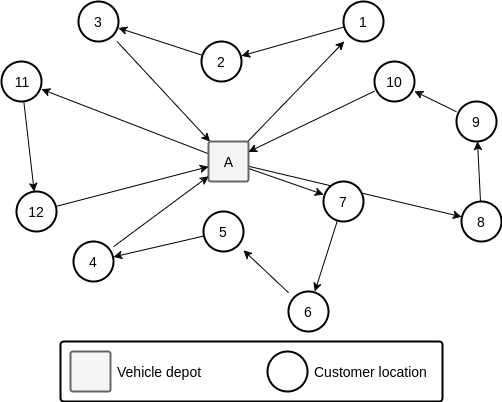
\includegraphics[width=9cm]{Resources/Images/vrp-ilustration}
	\captionsetup{format=hang}
	\caption{Ilustrasi \textit{Vehicle Routing Problem (VRP)}}
	\label{fig:vrp-ilustration}
\end{figure}


Terdapat sejumlah variasi dari VRP klasik yang telah diteliti, antara lain: \textit{Capacitated VRP (CVRP)} yang diteliti oleh \citep{baldacci_exact_2010}, \citep{cordeau_chapter_2007}, dan \citep{toth_vehicle_2002}; \textit{VRP with Time Windows (VRPTW)}, \textit{VRP with Pickup and Delivery (VRPPD)}, dan \textit{Periodic VRP (PVRP)} oleh \citep{solomon_survey_1988}; \textit{Dynamic VRP (DVRP)} oleh \citep{psaraftis_dynamic_1995}, dan berbagai varian lainnya, yang hanya mempertimbangkan satu buah depot. Sementara itu, \textit{Multi-Depot Vehicle Routing Problem (MDVRP)} merupakan salah satu varian dari VRP klasik yang menggunakan lebih dari satu depot. Gambar \ref{fig:vrp-variants} memberikan ilustrasi hierarki variasi dari VRP.


\begin{figure}[!]
	\centering
	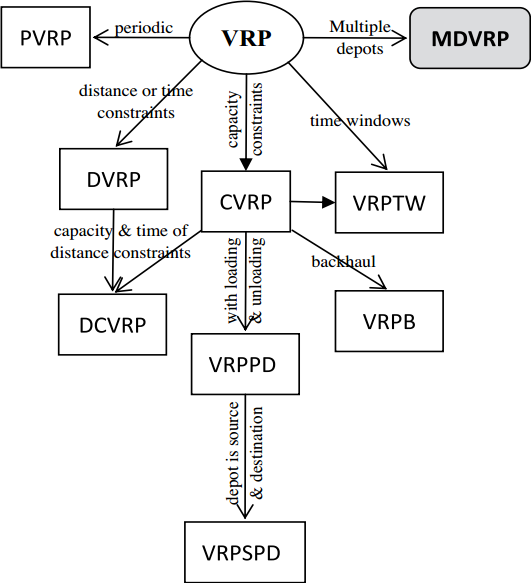
\includegraphics[width=8cm]{Resources/Images/vrp-variants}
	\captionsetup{format=hang}
	\caption{Hierarki variasi dari VRP \citep{weise_solving_2009}}
	\label{fig:vrp-variants}
\end{figure}


%-----------------------------------------------------------------------------%
\subsection{\textit{Multi-Depot Vehicle Routing Problem}}
\label{ssec:mdvrp}
%-----------------------------------------------------------------------------%
\textit{Multi-Depot Vehicle Routing Problem (MDVRP)} merupakan salah satu varian dari VRP klasik yang menggunakan lebih dari satu depot. Pada variasi ini, setiap pelanggan akan dikunjungi oleh kendaraan yang berasal dari salah satu dari beberapa depot. Pada MDVRP standar, kendaraan harus memulai dan mengakhiri rute pada depot yang sama. Gambar \ref{fig:mdvrp-illustration} memberikan ilustrasi tentang MDVRP.


\begin{figure}[!]
	\centering
	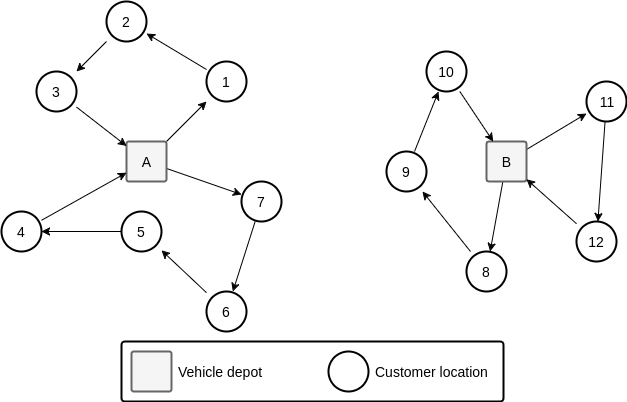
\includegraphics[width=11cm]{Resources/Images/mdvrp-illustration}
	\captionsetup{format=hang}
	\caption{Ilustrasi \textit{Multi Depot} VRP}
	\label{fig:mdvrp-illustration}
\end{figure}


Berdasarkan \citep{renaud_tabu_1996}, MDVRP dapat diformulasikan sebagai berikut, $G = (V, A)$ adalah sebuah \textit{graph}. $V$ adalah sebuah set dari simpul(\textit{vertex} atau \textit{node}) dan $A$ adalah sebuah set dari busur(\textit{arcs}). \textit{Node} dibagi menjadi 2 (dua) \textit{subset}: pelanggan yang akan dilayani $V_C$ = \{1,..., $N$\}, dan satu set depot $V_D$ = \{$N$+1,..., $N+M$\}, dan memiliki syarat $V_C \cup V_D$ = $V$ dan $V_C \cap V_D$ = $\oslash$. Terdapat biaya \textit{non-negative} $c_{ij}$ yang diasosiasikan untuk setiap \textit{arc} $(i, j) \in A$. \textit{Demand} untuk masing-masing pelanggan adalah $d_i$, dan tidak ada \textit{demand} pada \textit{depot node}. Terdapat juga sejumlah $K$ kendaraan yang identik, yang masing-masing memiliki kapasitas $Q$. \textit{Service time} untuk masing-masing pelanggan $i$ adalah $t_i$, sementara waktu durasi maksimum untuk masing-masing rute adalah $T$. Faktor konversi $w_{ij}$ mungkin dibutuhkan untuk menkonversi \textit{cost} $c_{ij}$ menjadi unit waktu. Pada MDVRP klasik, \textit{cost} sama dengan waktu dan unit jarak, sehingga $w_{ij}$ = $1$.


Dalam formula matematika, berdasarkan \citep{kulkarni_integer_1985}, variabel biner $x_{ijk}$ sama dengan $1$ ketika kendaraan $k$ mengunjungi \textit{node} $j$ tepat setelah \textit{node} $i$. Variabel tambahan $y_i$ juga digunakan untuk mengeliminasi \textit{subtour}. Persamaan \ref{eq:1} meminimalisasi \textit{total cost}. Persamaan \ref{eq:2} dan \ref{eq:3} menjamin bahwa setiap pelanggan hanya dilayani tepat satu kali oleh satu kendaraan. Alur kendaraan dijamin dengan persamaan \ref{eq:4}. Kapasitas kendaraan dan batasan durasi untuk setiap rute terdapat pada persamaan \ref{eq:5} and \ref{eq:6}. Persamaan \ref{eq:7} dan \ref{eq:8} mengecek keberadaan kendaraan. Eliminasi \textit{subtour} terdapat pada persamaan \ref{eq:9}. Terakhir, persamaan \ref{eq:10} dan \ref{eq:11} mendefinisikan $x$ dan $y$ sebagai variabel biner.


\begin{flalign}
\label{eq:1}
&\sum_{i=1}^{N+M}\sum_{j=1}^{N+M}\sum_{k=1}^{K}c_{ij}x_{ijk};
\end{flalign}


\begin{flalign}
\label{eq:2}
\sum_{i=1}^{N+M}\sum_{k=1}^{K}x_{ijk} = 1  (j=1,..., N);
\end{flalign}


\begin{flalign}
\label{eq:3}
\sum_{j=1}^{N+M}\sum_{k=1}^{K}x_{ijk} = 1  (j=1,..., N);
\end{flalign}


\begin{flalign}
\label{eq:4}
&\sum_{i=1}^{N+M}x_{ihk} - \sum_{j=1}^{N+M}x_{hjk} = 0 \\
\nonumber
&(k=1,...,K; h=1,...,N+M);
\end{flalign}


\begin{flalign}
\label{eq:5}
\sum_{i=1}^{N+M} \sum_{j=1}^{N+M} d_ix_{ijk} \leq Q (k=1,...,K);
\end{flalign}


\begin{flalign}
\label{eq:6}
\sum_{i=1}^{N+M} \sum_{j=1}^{N+M} (c_{ij}w_{ij} + t_i) x_{ijk} \leq T (k=1,...,K);
\end{flalign}


\begin{flalign}
\label{eq:7}
\sum_{i=N+1}^{N+M} \sum_{j=1}^{N} x_{ijk} \leq 1 (k=1,...,K);
\end{flalign}


\begin{flalign}
\label{eq:8}
\sum_{j=N+1}^{N+M} \sum_{i=1}^{N} x_{ijk} \leq 1 (k=1,...,K);
\end{flalign}


\begin{flalign}
\label{eq:9}
&y_i - y_j + (M + N)x_{ijk} \leq N + M - 1; \\
\nonumber
&for 1 \leq i \neq j \leq N and 1 \leq k \leq K;
\end{flalign}


\begin{flalign}
\label{eq:10}
x_{ijk} \in \{0, 1\} \forall i,j,k;
\end{flalign}


\begin{flalign}
\label{eq:11}
y_i \in \{0,1\} \forall i;
\end{flalign}


Terdapat beberapa algoritma yang dapat digunakan untuk menyelesaikan permasalahan MDVRP. \citep{laporte_optimal_1984} dan \citep{laporte_solving_1988} mengembangkan algoritma \textit{branch-and-bound}, tetapi, algoritma ini hanya dapat digunakan untuk sejumlah kecil \textit{instance}. Sejumlah algoritma \textit{heuristic} juga telah diteliti untuk MDVRP. Algoritma heuristic yang relatif awal, yang berbasis pada prosedur \textit{simple construction and improvement} diteliti oleh \citep{tillman_multiple_1969}, \citep{tillman_upperbound_1972}, \citep{tillman_study_1971}, \citep{wren_computer_1972}, \citep{gillett_multi-terminal_1976}, \citep{golden_implementing_1977}, dan \citep{raft_modular_1982}. Penelitian yang lebih baru, \citep{chao_new_1993} mengusulkan sebuah prosedur pencarian yang mengkombinasikan metode lokal \textit{record-to-record} \citep{dueck_new_1993} untuk mengalokasikan ulang pelanggan ke rute kendaraan yang berbeda, yang dilanjutkan dengan prosedur 2-opt \citep{lin_computer_1965} untuk meningkatkan rute individual.


Penelitian yang lain, \citep{renaud_tabu_1996} menggunakan \textit{tabu search heuristic}. solusi awal pada \textit{tabu search heuristic} disusun dengan meng-\textit{assign} setiap pelanggan dengan depot terdekatnya. Algoritma \textit{petal} yang dirancang oleh penulis yang sama, \citep{renaud_improved_1996}, kemudian digunakan untuk mencari solusi dari setiap VRP yang diasosiasikan pada masing-masing depot. Terakhir terdapat fase \textit{improvement}, baik dengan menggunakan subset dari pertukaran 4-opt untuk meningkatkan rute individual, menukar pelanggan antar rute dari depot yang sama maupun berbeda, atau menukar pelanggan antara 3 (tiga) rute.


Penggunaan \textit{tabu search} juga dilakukan oleh \citep{cordeau_tabu_1997}. Solusi awal pada \textit{tabu search} diperoleh dengan memetakan setiap pelanggan dengan depot terdekat dan solusi digenerate untuk masing-masing depot dengan menggunakan algoritma sweep. \textit{Improvement} dilakukan dengan memindahkan pelanggan antara dua rute kepada depot yang sama, atau dengan merelokasi pelanggan pada rute ke depot yang lain. \textit{Reinsertion} dilakukan dengan menggunakan \textit{GENI heuristic} \citep{gendreau_new_1992}.


Selain tabu search, terdapat juga beberapa algoritma yang dapat digunakan untuk menyelesaikan permasalahan MDVRP, yaitu: adaptive large neighborhood search (ALNS) \citep{pisinger_general_2007}, fuzzy logic guided genetic algorithm (FLGA) \citep{lau_application_2010}, paralel iterated tabu search (ITS) \citep{cordeau_parallel_2012}, hybrid algorithm combining Iterated Local Search and Set Partitioning (ILS-RVND-SP) \citep{subramanian_hybrid_2013}, hybrid genetic algorithm with adaptive diversity control (HGSADC+) \citep{vidal_implicit_2014}, hybrid Granular Tabu Search (ELTG) \citep{escobar_hybrid_2014}, dan evolution algorithms (EAs) \citep{weise_solving_2009}.


%-----------------------------------------------------------------------------%
\subsection{\textit{Cooperative Evolution Strategy}}
\label{ssec:coes}
%-----------------------------------------------------------------------------%
\textit{Evolution Strategies (ESs)} merupakan salah satu \textit{family} dari algoritma optimasi yang terinspirasi dari alam. ESs pertama kali diteliti oleh \citep{rechenberg_cybernetic_1965} dan \citep{huning_evolutionsstrategie._1976}, yang kemudian diteliti lebih lanjut oleh \citep{schwefel_evolutionsstrategie_1975}. Pada ESs, setiap individu direpresentasikan oleh \textit{genetic building blocks} dan parameter strategi yang memodelkan perilaku individu pada lingkungannya. Evolusi kemudian terjadi, yang terdiri dari perkembangan dari karakteristik genetik dan parameter strategi. Evolusi dari karakterisik genetik dikontrol oleh parameter strategi.


ESs merepresentasikan individu sebagai sebuah \textit{tuple}, yang terdiri dari \textit{decision vector} $x$ yang akan dioptimalisasi, dan vector parameter strategi $\sigma$ yang merepresentasikan jumlah mutasi dari setiap dimensi.


\begin{flalign}
\chi(t) = (x(t), \sigma(t))
\end{flalign}


Berdasarkan observasi biologi, keturunan (\textit{offspring}) harus mempunyai kesamaan dengan induknya, 


\begin{flalign}
\chi'(t) = (x'(t), \sigma'(t))
\end{flalign}


Operator seleksi kemudian akan menentukan yang terbaik antara induk dan keturunannnya. Asumsi yang digunakan adalah, 


\begin{flalign}
x(t+1) = \left\{\begin{matrix}x'(t) &f(x'(t)) < f(x(t)) \\ 
x(t) &otherwise\end{matrix}\right.
\end{flalign}


dan 


\begin{flalign}
\sigma(t+1) = \left\{\begin{matrix}\sigma'(t) &f(x'(t)) < f(x(t)) \\ 
\sigma(t) &otherwise\end{matrix}\right.
\end{flalign}


Algoritma \ref{alg:es} merupakan framework generik pada implementasi ES. Parameter $\mu$ and $\lambda$ mengindikasikan jumlah induk dan jumlah keturunannya. Komponen utama dari algoritma ES adalah:

\begin{enumerate}
\item \textbf{Initialization:} Untuk setiap individu, \textit{genotype}-nya diinisialisasi sesuai dengan konstrain dari masalah. Parameter dari strategi juga diinisialisasi.
\item \textbf{Recombination:} Keturunan diproduksi dengan melalui operator \textit{crossover} pada dua atau lebih induk.
\item \textbf{Mutation:} Keturunan kemudian bermutasi, yang jumlah mutasinya diukur dari parameter strategi adaptasi.
\item \textbf{Evaluation:} \textit{Absolute fitness function} digunakan untuk mengukur kualitas dari solusi yang direpresentasikan dengan \textit{genotype} dari individu.
\item \textbf{Selection:} Operator seleksi digunakan untuk dua tujuan: memilih induk untuk rekomendasi, dan menentukan individu yang masih bertahan.
\end{enumerate}


\begin{algorithm}[!]
	\captionsetup{format=hang}
	\caption{Algoritma Evolution Strategy}
	\label{alg:es}
	\begin{algorithmic}[1]
		\STATE Set the generation counter, $t = 0$;
		\STATE Initialize the strategy parameters;
		\STATE Create and initialize the population, $C(0)$, of $\mu$ individuals;
		\FOR {each individual, $\chi_i(t) \in C(t)$}
			\STATE Evaluate the fitness, $f(x_i(t))$;
		\ENDFOR
		\WHILE {stopping condition(s) not true}
			\FOR {$i = 1,...,\lambda$}
				\STATE Choose $\rho \geq 2$ parents at random;
				\STATE Create offspring through application of crossover operator on parent genotypes and strategy parameters;
				\STATE Mutate offspring strategy parameters and genotype;
				\STATE Evaluate the fitness of the offspring;
			\ENDFOR
			\STATE Select the new population, $C(t + 1)$;
			\STATE $t = t + 1$;
		\ENDWHILE
	\end{algorithmic}
\end{algorithm}


Jika \textit{evolution algorithm} (EA) memandang evolusi hanya sebagai suatu usaha populasi untuk beradaptasi dengan lingkungan yang tetap, maka algoritma \textit{coevolution} (CoEA) memandang evolusi dari pendekatan yang lebih bersifat natural dengan memperhatikan hubungan yang saling melengkapi (komplemen) antara spesies terkait. Ilustrasi \textit{coevolution} antara dua spesies adalah seperti dicontohkan oleh \citep{holland_echo:_1990}, yaitu interaksi antara tanaman dan serangga. Agar tetap dapat bertahan, tanaman membutuhkan mekanisme evolusi untuk mempertahankan diri dari serangga, sementara serangga membutuhkan tanaman sebagai sumber makanan. Keduanya, tanaman dan serangga, masing-masing berevolusi untuk memdapatkan karakteristik yang membuat mereka bertahan hidup.


Perbedaan antara algoritma CoEA dengan EA adalah CoEA tidak hanya terkait antar populasi, tetapi juga merespon perubahan lingkungan yang disebabkan oleh populasi yang lain. Perbedaan lain yang cukup signifikan adalah EA mendefinisikan solusi optimal melalui fungsi \textit{fitness} yang bersifat absolut yang mendorong terjadinya evolusi. Sebaliknya, CoEA tidak mendefinisikan fungsi \textit{fitness}, sehingga proses evolusi terus berlangsung. Solusi yang paling optimal diperoleh dengan cara mengalahkan lawan.


Terdapat dua macam pendekatan berbasis \textit{coevolution}, yaitu \textit{competitive coevolution} dan \textit{cooperative coevolution}. \textit{Competitive coevolution} dibagi menjadi dua: 1) \textbf{Competition}, yaitu kondisi ketika satu atau lebih populasi saling menghambat. Keberhasilan satu populasi membuat populasi lain gagal. 2) \textbf{Amensalism}, yaitu kondisi ketika terhambatnya satu populasi tidak berpengaruh terhadap populasi lain. Sementara  \textit{cooperative coevolution} juga dibagi menjadi tiga: 1) \textbf{Mutualism}, yaitu kondisi ketika satu atau lebih populasi saling menguntungkan. 2) \textbf{Commensalism}, yaitu kondisi ketika hanya sebagian populasi diuntungkan, sementara populasi yang lain tidak terpengaruh. 3) \textbf{Parasitism}, yaitu kondisi ketika sebagian populasi mengambil keuntungan dari populasi yang lain.


Penelitian yang menggunakan CoEA, dalam kaitannya dengan penyelesaian masalah MDVRP, salah satunya dilakukan oleh \citep{de_oliveira_cooperative_2016}. \citep{de_oliveira_cooperative_2016} membagi masalah menjadi beberapa submasalah. Tiap-tiap submasalah akan menjadi sebuah populasi yang akan berinteraksi dengan populasi yang lain. Setiap populasi kemudian akan berevolusi. Sebagaimana pada teori \textit{coevolution}, evolusi dari satu populasi akan mempengaruhi populasi yang lain. Pada penelitian \citep{de_oliveira_cooperative_2016}, hubungan yang terjadi pada setiap populasi bersifat kooperatif. Seluruh populasi akan saling bekerja sama membentuk solusi terbaik.


\begin{figure}[!]
	\centering
	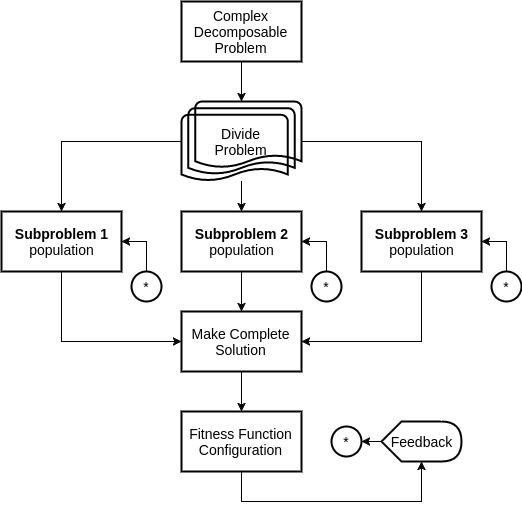
\includegraphics[width=10cm]{Resources/Images/coes_overview}
	\captionsetup{format=hang}
	\caption{\textit{Lifecycle} pada \textit{Cooperative Coevolution} \citep{de_oliveira_cooperative_2016}}
	\label{fig:coes_lifecycle}
\end{figure}


%-----------------------------------------------------------------------------%
\section{Messaging Solution}
\label{sec:messaging-solution}
%-----------------------------------------------------------------------------%


Ketika dua buah aplikasi ingin saling bertukar data, mereka akan melakukannya dengan mengirimkan data melalui \textit{channel} yang akan menghubungkan keduanya. Yang menjadi tantangan adalah memilih mekanisme yang tepat dalam pengiriman pesan.


Dari beragam metode interaksi antara \textit{client} dengan \textit{server}, cara yang paling banyak digunakan adalah dengan melalui media web. Hal senada juga terjadi dalam implementasi \textit{location routing problem} yang sebagian besar menggunakan media web, seperti \citep{weise_solving_2009}, \citep{sengoku_fast_1998}, \citep{sarmenta_bayanihan_2002}, dan \citep{diaz_vrp_2012}. Akan tetapi, teknologi web bekerja secara \textit{synchronous}, yaitu setiap \textit{request} dan \textit{reply} akan diproses secara berurutan, sehingga tidak sesuai untuk diimplementasikan pada sistem yang bersifat \textit{information driven} \citep{muhl_large-scale_2002}. Selain itu, komunikasi \textit{point-to-point} dan \textit{synchronous} membuat pengembangan menjadi tidak fleksibel \citep{eugster_many_2003}.


%-----------------------------------------------------------------------------%
\subsection{Mekanisme \textit{Publish/Subscribe}}
\label{ssec:pub-sub-mechanism}
%-----------------------------------------------------------------------------%
\textit{Publish/subscribe interaction} merupakan salah satu alternatif untuk komunikasi antara \textit{client} dan \textit{server}. Paradigma interaksi pada \textit{publish/subscribe} adalah adanya \textit{subscriber} yang memiliki ketertarikan pada suatu \textit{event} atau \textit{pattern of event} dan ingin mendapatkan notifikasi tiap kali \textit{event} yang menjadi \textit{interest}-nya di-\textit{publish} oleh \textit{publisher}.


Model dasar dari sistem berbasis \textit{publish/subscribe}, seperti Gambar \ref{fig:pub-sub-general}, bergantung pada \textit{event notification service} yang menyediakan penyimpanan dan manajemen dari \textit{subscription}. \textit{Event service} tersebut berperan sebagai mediator antara \textit{publisher} yang berperan sebagai produsen \textit{event} dan \textit{subscriber} yang berperan sebagai konsumen dari \textit{event}. 


\textit{Subscriber} mendaftarkan ketertarikannya pada sebuah \textit{event} tanpa perlu mengetahui sumber dari \textit{event} tersebut, dengan memanggil operasi \textit{subscribe()} pada \textit{event service}. Informasi \textit{subscription} ini tetap tersimpan di dalam penyimpanan pada \textit{event service}. Untuk menciptakan \textit{event}, \textit{publisher} memanggil operasi \textit{publish()}. \textit{Event service} kemudian meneruskan \textit{event} yang diproduksi tersebut kepada \textit{subscriber} yang bersesuaian.


\begin{figure}[!]
	\centering
	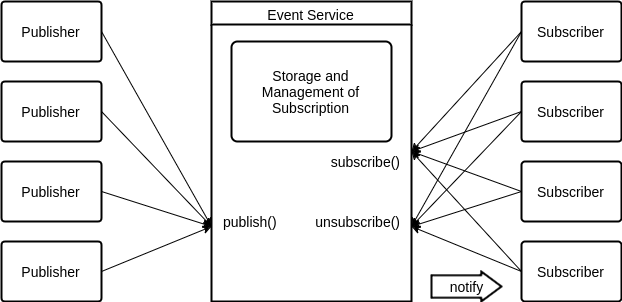
\includegraphics[width=11cm]{Resources/Images/pub-sub-general}
	\captionsetup{format=hang}
	\caption{Arsitektur dasar pada Pub/Sub \citep{eugster_many_2003}}
	\label{fig:pub-sub-general}
\end{figure}


Paradigma \textit{publish/subscribe} memiliki sifat \textit{loose coupling}. Pemisahan (\textit{decoupling}) informasi yang terjadi antara \textit{subscriber} dan \textit{publisher} dapat dibedakan ke dalam 3 (tiga) dimensi, sebagaimana diilustrasikan pada Gambar \ref{fig:space-time-sync-decoupling}. \textit{Decoupling} informasi tersebut berlangsung sebagai berikut:

\begin{enumerate}
\item \textit{Space decoupling.} \\
Interaksi antara \textit{publisher} dan \textit{subscriber} tidak perlu saling mengetahui satu dengan yang lain. \textit{Publisher} mengirimkan \textit{event}, dan \textit{subscriber} menerima \textit{event} secara tidak langsung melalui \textit{event service}. \textit{Publisher} biasanya tidak memiliki referensi tentang \textit{subscriber}. Begitu juga sebaliknya, \textit{subscriber} biasanya tidak memegang referensi tentang \textit{publisher}.
\item \textit{Time decoupling.} \\
Pihak-pihak yang berinteraksi tidak harus berinteraksi pada waktu yang bersamaan. \textit{Publisher} dapat mengirimkan \textit{event} pada saat \textit{subscriber} dalam kondisi terputus (\textit{offline}). Begitu juga sebaliknya, \textit{subscriber} tetap dapat menerima \textit{event}, meskipun \textit{original publisher} sedang dalam kondisi terputus (\textit{offline}).
\item \textit{Synchronizing decoupling.} \\
\textit{Publisher} dan \textit{subscriber} tidak berada dalam \textit{main flow}, sehingga tidak berinteraksi secara \textit{synchronous}. \textit{Publisher} tetap dapat mengirimkan informasi meskipun sedang memproduksi \textit{event} lain dan \textit{subscriber} tetap dapat memperoleh informasi meskipun sedang mengerjakan tugas yang lain. 
\end{enumerate}


\begin{figure}[!]
	\centering
	\begin{subfigure}[t]{9cm}
		\centering
		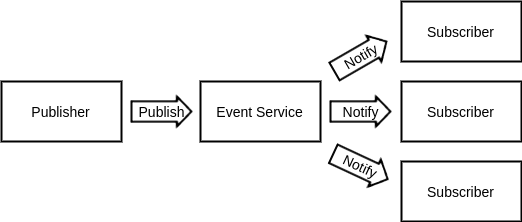
\includegraphics[width=\textwidth]{Resources/Images/space-decoupling}
		\caption{\textit{Space Decoupling}}
		\label{fig:space-decoupling}
	\end{subfigure}%
	
	\begin{subfigure}[t]{10cm}
		\centering
		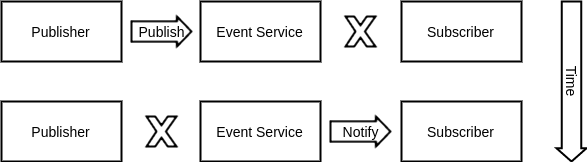
\includegraphics[width=\textwidth]{Resources/Images/time-decoupling}
		\caption{\textit{Time Decoupling}}
		\label{fig:time-decoupling}
	\end{subfigure}%
	
	\begin{subfigure}[t]{9cm}
		\centering
		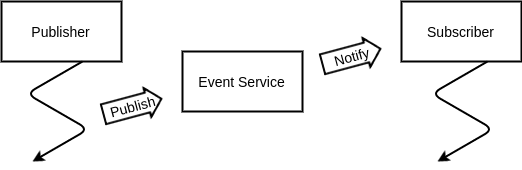
\includegraphics[width=\textwidth]{Resources/Images/sync-decoupling}
		\caption{\textit{Sync Decoupling}}
		\label{fig:sync-decoupling}
	\end{subfigure}
	\captionsetup{format=hang}
	\caption{Pemisahan informasi pada Pub/Sub \citep{eugster_many_2003}}
	\label{fig:space-time-sync-decoupling}
\end{figure}
